
% RECONSTRUCTION GRAPH
\begin{tikzpicture}[node distance=1cm and 1.7cm, auto]
%%Nodes

\node (D) [minimum height=3.5cm] {\distribution};
\node [above of= D, align=center, yshift=0.7cm] {data set \\ distribution};

\node (A) [node, right= 1cm of D, fill=red!7, yshift=2cm] {\textbf{target} \\ $\set A$};
\node (B) [node, right= 1cm of D, yshift=-2cm] {\textbf{original} \\ $\set B_\text{true}$};

\node (Bp) [node, right= of B, fill=blue!3] {perturbed \\ \textbf{source} \\ $\set B$}; %\\ $\set B = \delta (\set B_\text{true})$};
\node (Br) [node, right= of Bp, fill=blue!7] {\textbf{reconstructed} \\ $\rho (\set B)$};


%%Arrows
\draw [arrow, dashed, thin] (D) -- (A.190);
\draw [arrow, dashed, thin] (D) -- (B.170);


\draw [arrow, dashed, thin] (B) -- (Bp) 
node (Pert) [midway, function, dashed] {$\delta$};
\draw [linestart] (Bp) -- (Br) 
node (Rec) [midway, function, draw=blue, fill=white] {$\rho$};
\node [fill=white, below= 0cm of Rec] {\color{blue} \footnotesize optimize};
\node [fill=white, below= 0cm of Pert] {\footnotesize \textit{unknown}};


% \draw [dashed] (Rec) to [out=245, in=115] (Rec2);

\node (Net) [function, thick, minimum width= 1cm, above right= -0cm and 3.1cm of A] {$\varphi$};
\node [above right=-0.2cm and 0cm of Net] {\small feature-map};
\node (Loss) [function, thick, above= 1.5cm of Net] {loss};

\pgfmathtruncatemacro{\OutL}{110}
\pgfmathtruncatemacro{\OutM}{95}
\pgfmathtruncatemacro{\OutR}{75}
\pgfmathtruncatemacro{\InL}{360-\OutL}
\pgfmathtruncatemacro{\InM}{360-\OutM}
\pgfmathtruncatemacro{\InR}{360-\OutR}

\draw [lineend] (Net.\InL) to [corner connect h=-0.7cm] (A.east);
\draw [arrowend] (Net.\OutL) to [out=90, in=270] (Loss.260);

\draw [line] (Net.\InM) to [rect connect h=-0.7cm] (Br.100);
\draw [arrowend] (Net.\OutM) to [out=90, in=270] (Loss.260);

\draw [line, blue] (Net.\InR) to [rect connect h=-0.4cm] (Br.80);
\draw [lineend, blue, connect v] (Net.\OutR) to (Loss.south);
\draw [arrowend, blue, connect h] (Br.192) to (Rec.east);

\path (Net.\OutL) -- node[midway, above= 0.15cm, sloped] {\small statistics}(Loss.260);
% \node [above= 0.5cm of Net, fill=white] {\footnotesize optimize};
% \draw [arrow, Mahogany, thin, bend left=20] (A) to node[near end, above] {\footnotesize trained} (Net);

\setlength{\fboxsep}{0pt}%
\setlength{\fboxrule}{1pt}%

\node [below= 0cm of A] {\fbox{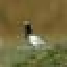
\includegraphics[]{figures/CIFAR10_example_2.pdf}}};
\node [below= 0cm of B] {\fbox{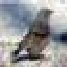
\includegraphics[]{figures/CIFAR10_example.pdf}}};
\node [below= 0cm of Bp] {\fbox{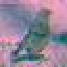
\includegraphics[]{figures/CIFAR10_example_distort.pdf}}};
\node [below= 0cm of Br] {\fbox{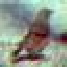
\includegraphics[]{figures/CIFAR10_example_reconstruct.pdf}}};

\end{tikzpicture}




% % RECONSTRUCTION GRAPH
% \begin{tikzpicture}[node distance=1cm and 1.7cm, auto]
% %%Nodes

% \node (D) [minimum height=3.5cm] {\distribution};
% \node [above of= D, align=center, yshift=0.7cm] {data set \\ distribution};

% \node (A) [node, right= 1cm of D, fill=red!7, yshift=1.5cm] {\textbf{target} \\ $\set A$};
% \node (B) [node, right= 1cm of D, yshift=-1.5cm] {\textbf{original} \\ $\set B_\text{true}$}

% \node (Bp) [node, right= of B, fill=blue!3] {perturbed \\ \textbf{source} \\ $\set B$}; %\\ $\set B = \delta (\set B_\text{true})$};
% \node (Br) [node, right= of Bp, fill=blue!7] {\textbf{reconstructed} \\ $\rho (\set B)$};


% %%Arrows
% \draw [arrow, dashed, thin] (D) -- (A.190);
% \draw [arrow, dashed, thin] (D) -- (B.170);


% \draw [arrow, dashed, thin] (B) -- (Bp) 
% node (Pert) [midway, function, dashed] {$\delta$};
% \draw [linestart] (Bp) -- (Br) 
% node (Rec) [midway, function, draw=blue, fill=white] {$\rho$};
% \node [fill=white, below= 0cm of Rec] {\color{blue} \footnotesize optimize};
% \node [fill=white, below= 0cm of Pert] {\footnotesize \textit{unknown}};


% % \draw [dashed] (Rec) to [out=245, in=115] (Rec2);

% \node (Net) [function, thick, minimum width= 1cm, above right= -0cm and 3.1cm of A] {$\varphi$};
% \node [above right=-0.2cm and 0cm of Net] {\small feature-map};
% \node (Loss) [function, thick, above= 1.5cm of Net] {loss};

% \pgfmathtruncatemacro{\OutL}{110}
% \pgfmathtruncatemacro{\OutM}{95}
% \pgfmathtruncatemacro{\OutR}{75}
% \pgfmathtruncatemacro{\InL}{360-\OutL}
% \pgfmathtruncatemacro{\InM}{360-\OutM}
% \pgfmathtruncatemacro{\InR}{360-\OutR}

% \draw [lineend] (Net.\InL) to [corner connect h=-0.7cm] (A.east);
% \draw [arrowend] (Net.\OutL) to [out=90, in=270] (Loss.260);

% \draw [line] (Net.\InM) to [rect connect h=-0.7cm] (Br.100);
% \draw [arrowend] (Net.\OutM) to [out=90, in=270] (Loss.260);

% \draw [line, blue] (Net.\InR) to [rect connect h=-0.4cm] (Br.80);
% \draw [lineend, blue, connect v] (Net.\OutR) to (Loss.south);
% \draw [arrowend, blue, connect h] (Br.192) to (Rec.east);

% \path (Net.\OutL) -- node[midway, above= 0.15cm, sloped] {\small statistics}(Loss.260);
% % \node [above= 0.5cm of Net, fill=white] {\footnotesize optimize};
% % \draw [arrow, Mahogany, thin, bend left=20] (A) to node[near end, above] {\footnotesize trained} (Net);


% \end{tikzpicture}

